\chapter{Deployment}

\begin{figure}[hbtp]
	\centering
	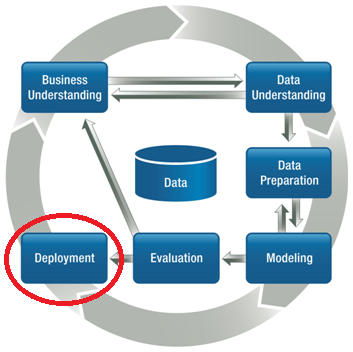
\includegraphics[width=0.5\textwidth]{./images/CRISPDM_6.png}
	\caption{CRISP-DM - Deployment}
	\label{CRISPDM_6}
\end{figure}
\section{Piano di Deployment}
Considerato il fatto che i risultati ottenuti hanno confermato il superamento degli obiettivi di business definiti dal progetto, possiamo prendere in considerazione il fatto di poter utilizzare la configurazione migliore ottenuta come un ulteriore filtro anti-spam da poter utilizzare in un gestore di posta elettronica reale quale Microsoft Outlook o Mozilla Thunderbird.
%Il filtro anti spam creato, visti i risultati positivi ottenuti, può essere utilizzato come ulteriore filtro ai già presenti filtri integrati nei principali gestori di posta elettronica, quali outlook e thunderbird.
\section{Monitoraggio e Manutenzione}
Al fine di poter essere utilizzabile per molto tempo, diviene necessario manuntenere il sistema raffinandolo attraverso l'ausilio di un quantitativo maggiore di email in modo tale da riuscire a catturare anche le nuove tipologie di spam.
